\chapter{Performance}
\label{chap:perfux}
All measurements were made on hardware with following characteristics:
\begin{itemize}
	\item Mac mini (Late 2014)
	\item \textbf{Processor:} 2.6 GHz Intel Core i5;
	\item \textbf{Memory:} 8 GB 1600 MHz DD3;
	\item \textbf{Storage:}  1 TB SATA Disk.
\end{itemize}

Operational System:
\begin{itemize}
	\item OS X El Capitan
	\item version 10.11.4
\end{itemize}


\section{Generation performance}
\paragraph{Single folder} - all files are located within same folder (Diagram: \ref{fig:gs}).
\begin{itemize}
	\item \textbf{Add} - 10 .xlsx files are added on every iteration of the measurement processes. Thus previously added xlsx files were skipped for js files creation. All js files were skipped. 10 xlsx files read and 10 js generated;
	\item \textbf{New} - all the files are newly added on the every iteration of the measurement with deletion of previously generated .js files. Thus the number of generated js files is equivalent to the number of files in a directory.
\end{itemize}


\begin{figure}[ht]
	\label{fig:gs}
	\centering
	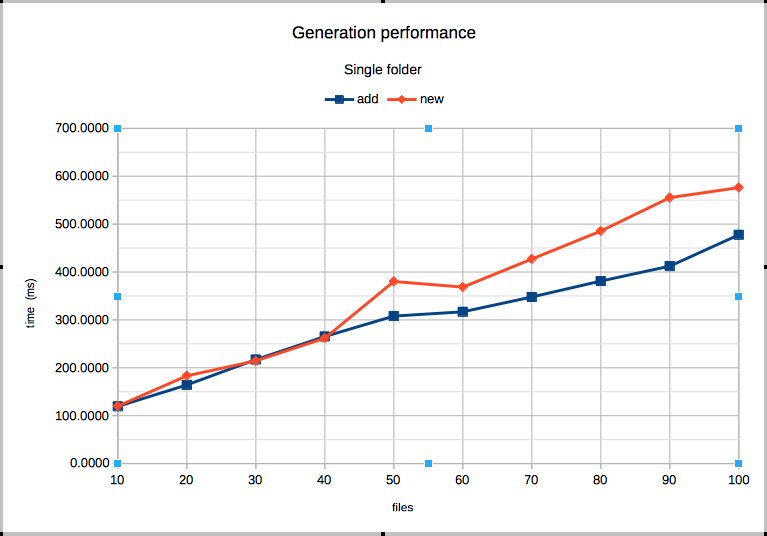
\includegraphics[width=\textwidth]{grafiken/generation_single}
	\caption{Generation performance for files within single folder}
\end{figure}

\paragraph{Nested folder} - each folder contains 10 .xlsx files and folder with the same content (Diagram: \ref{fig:gn}).
\begin{itemize}
	\item \textbf{Add} - 10 .xlsx files into the folder nested within the folder created inside the folder from the previous iteration are added . Thus previously added .xlsx files are skipped for  the .js files creation. All the .js files were skipped (10 .xlsx files read and 10 .js generated);
	\item \textbf{New} - all the files are newly added on the every iteration of the measurement with deletion of previously generated .js files but with nesting by 10 .xlsx files in each nested folder. Thus the number of generated js files is equivalent to the number of files in a directory.
\end{itemize}


\begin{figure}[ht]
	\label{fig:gn}
	\centering
	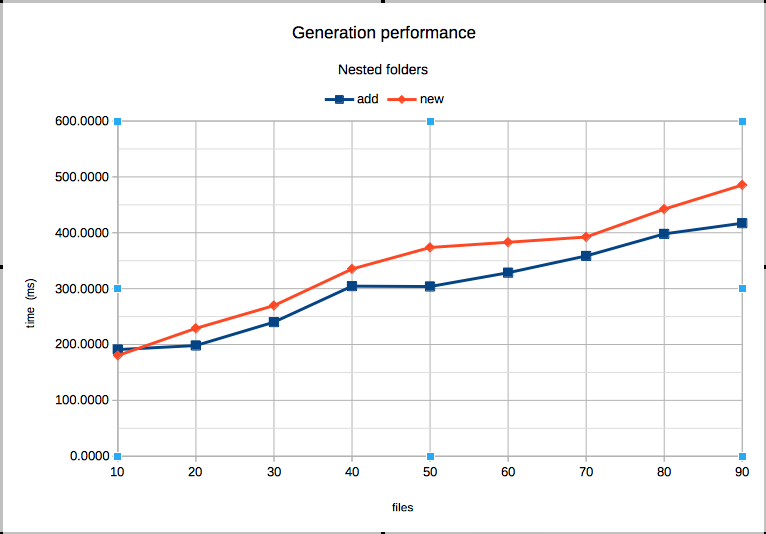
\includegraphics[width=\textwidth]{grafiken/generation_nested}
	\caption{Generation performance for files within nested folders}
\end{figure}

\section{Executions performance}
All the files are located within same folder 
\paragraph{Independent test steps} - all test steps are independent from each other and their call is done within the same iteration of an event loop (Diagram: \ref{fig:ei}).
\begin{itemize}
	\item \textbf{Scheme comparison} - actual and expected outputs are compared by their scheme
	\item \textbf{Deep comparison} - actual and expected outputs are compared by their scheme and values of every property
\end{itemize}
\begin{figure}[ht]
	\label{fig:ei}
	\centering
	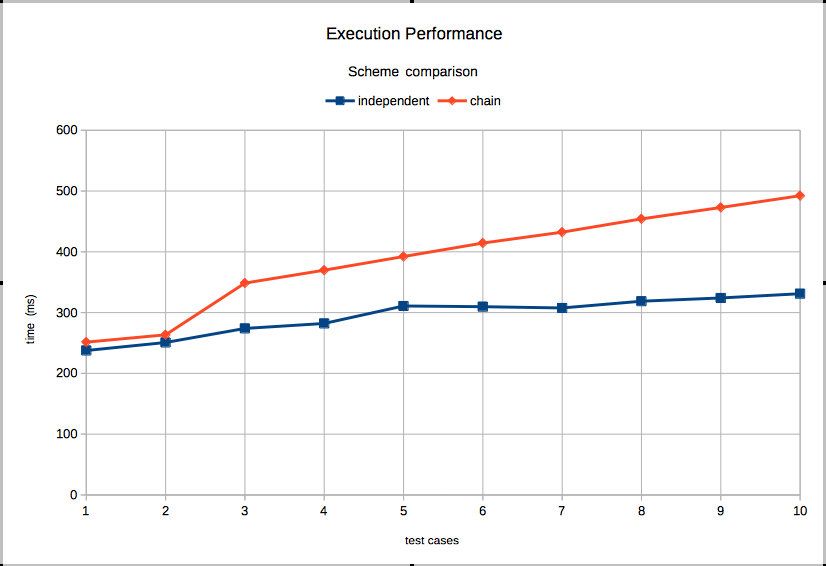
\includegraphics[width=\textwidth]{grafiken/exec_scheme}
	\caption{Execution performance for independent test steps}
\end{figure}

\paragraph{Chain relationship} - output of each row defines input for row below (Diagram: \ref{fig:ef}).
\begin{itemize}
	\item \textbf{Scheme comparison} - actual and expected outputs are compared by their scheme
	\item \textbf{Deep comparison} - actual and expected outputs are compared by their scheme and values of every property
\end{itemize}

\begin{figure}[ht]
	\label{fig:ef}
	\centering
	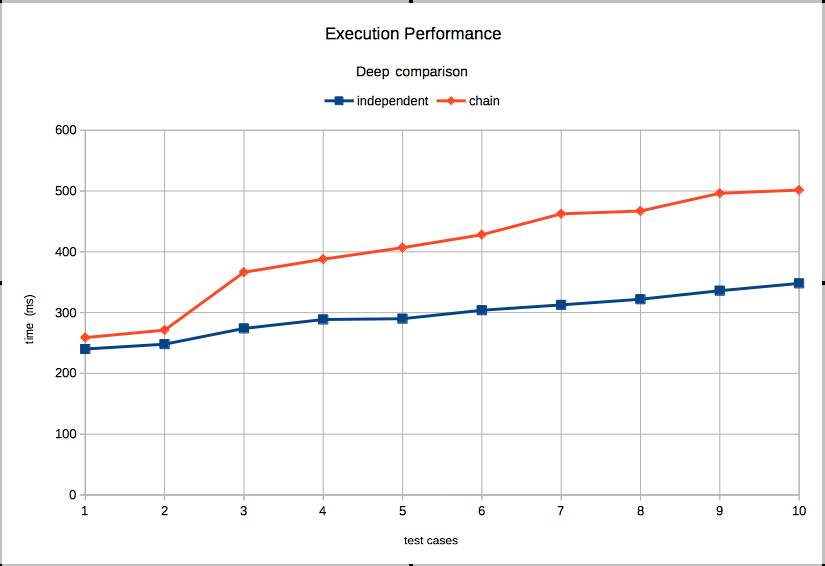
\includegraphics[width=\textwidth]{grafiken/exec_deep}
	\caption{Execution performance for interdependent test steps}
\end{figure}

